\documentclass{report}
\usepackage[top=3cm, bottom=3cm, left=3.5cm, right=3cm]{geometry}
\usepackage{tabularx}
\usepackage{float}
\usepackage{tikz}
\usepackage{longtable}
\usepackage{environ}
\usepackage{boldline}
\usepackage{circuitikz}
\frenchspacing

\usetikzlibrary{positioning, calc}

\newcounter{magicrownumbers}
\newcommand\rownumber{\stepcounter{magicrownumbers}\arabic{magicrownumbers}}

% ---------------
% Circuitikz symbols
% ---------------
\usepackage{tikz}
\usepackage{circuitikz}

\usetikzlibrary{calc}

% ---------------
% Example IC
% ---------------
\pgfdeclareshape{ic8pin}{
\anchor{center}{\pgfpointorigin} % (0,0) is the center

\anchor{text}
{\pgfpoint{-0.5\wd\pgfnodeparttextbox}{-.5\ht\pgfnodeparttextbox}}

\savedanchor\icpina{\pgfpoint{-.75cm}{-.625cm}}
\anchor{p1}{\icpina}
\savedanchor\icpinb{\pgfpoint{-.25cm}{-.625cm}} % pin 2
\anchor{p2}{\icpinb}
\savedanchor\icpinc{\pgfpoint{.25cm}{-.625cm}} % pin 3
\anchor{p3}{\icpinc}
\savedanchor\icpind{\pgfpoint{.75cm}{-.625cm}} % pin 4
\anchor{p4}{\icpind}
\savedanchor\icpine{\pgfpoint{.75cm}{.625cm}} % pin 5
\anchor{p5}{\icpine}
\savedanchor\icpinf{\pgfpoint{.25cm}{.625cm}} % pin 6
\anchor{p6}{\icpinf}
\savedanchor\icping{\pgfpoint{-.25cm}{.625cm}} % pin 7
\anchor{p7}{\icping}
\savedanchor\icpinh{\pgfpoint{-.75cm}{.625cm}} % pin 8
\anchor{p8}{\icpinh}


\foregroundpath{ % border and pin numbers are drawn here
\pgfsetlinewidth{0.05cm}
\pgfpathrectanglecorners{\pgfpoint{1cm}{.625cm}}{\pgfpoint{-1cm}{-.625cm}}
\pgfusepath{draw} %draw rectangle
\pgfsetlinewidth{0.03cm}
\pgfpathmoveto{\pgfpoint{-1cm}{-.3cm}}
\pgfpatharc{-90}{90}{.3cm}
\pgfusepath{draw} %draw semicircle
\pgftext[bottom,at={\pgfpoint{-.75cm}{-.55cm}}]{\scriptsize 1}
\pgftext[bottom,at={\pgfpoint{-.25cm}{-.55cm}}]{\scriptsize 2}
\pgftext[bottom,at={\pgfpoint{.25cm}{-.55cm}}]{\scriptsize 3}
\pgftext[bottom,at={\pgfpoint{.75cm}{-.55cm}}]{\scriptsize 4}
\pgftext[top,at={\pgfpoint{.75cm}{.55cm}}]{\scriptsize 5}
\pgftext[top,at={\pgfpoint{.25cm}{.55cm}}]{\scriptsize 6}
\pgftext[top,at={\pgfpoint{-.25cm}{.55cm}}]{\scriptsize 7}
\pgftext[top,at={\pgfpoint{-.75cm}{.55cm}}]{\scriptsize 8}
}}

% ---------------
% D FlipFlop
% ---------------
\pgfpoint{-.625cm}{.6cm}
\pgfgetlastxy{\xd}{\yd}
\pgfpoint{-.625cm}{-.6cm}
\pgfgetlastxy{\xc}{\yc}
\pgfpoint{.625cm}{.6cm}
\pgfgetlastxy{\xq}{\yq}
\pgfpoint{.625cm}{-.6cm}
\pgfgetlastxy{\xqn}{\yqn}
\pgfpoint{-.625cm}{-1cm}
\pgfgetlastxy{\xsw}{\ysw}
\pgfpoint{.625cm}{1cm}
\pgfgetlastxy{\xne}{\yne}

\pgfdeclareshape{dff}{
    \anchor{center}{\pgfpointorigin}

    \savedanchor\pind{\pgfpoint{\xd - 0.5cm}{\yd}}
    \anchor{d}{\pind}
    \savedanchor\pinc{\pgfpoint{\xc - 0.5cm}{\yc}}
    \anchor{c}{\pinc}
    \savedanchor\pinq{\pgfpoint{\xq + 0.5cm}{\yq}}
    \anchor{q}{\pinq}
    \savedanchor\pinnq{\pgfpoint{\xqn + 0.5cm}{\yqn}}
    \anchor{nq}{\pinnq}

    \foregroundpath{
        \pgfsetlinewidth{0.8pt}
        \pgfpathrectanglecorners{\pgfpoint{-.625cm}{-1cm}}{\pgfpoint{.625cm}{1cm}}
        \pgfusepath{draw}

        \pgfsetlinewidth{0.4pt}
        \pgftext[left,at={\pgfpoint{\xd + .1cm}{\yd}}]{\scriptsize $D$}
        \draw (\xd,\yd) -- ++(-0.5cm,0);

        \pgftext[left,at={\pgfpoint{\xc + .1cm}{\yc}}]{\scriptsize $C$}
        \draw (\xc,\yc) -- ++(-0.5cm,0);

        \pgftext[right,at={\pgfpoint{\xq - .1cm}{\yq}}]{\scriptsize $Q$}
        \draw (\xq,\yq) -- ++(0.5cm,0);

        \pgftext[right,at={\pgfpoint{\xqn - .1cm}{\yqn}}]{\scriptsize $\overline{Q}$}
        \draw (\xqn,\yqn) -- ++(0.5cm,0);
    }
}

% ---------------
% MUX
% ---------------
\pgfpoint{-.3cm}{-.55cm}
\pgfgetlastxy{\xl}{\yl}
\pgfpoint{-.3cm}{.55cm}
\pgfgetlastxy{\xu}{\yu}
\pgfpoint{0cm}{0.85cm}
\pgfgetlastxy{\xs}{\ys}
\pgfpoint{.3cm}{0cm}
\pgfgetlastxy{\xout}{\yout}

\pgfdeclareshape{mux}{
    \anchor{center}{\pgfpointorigin}

    \savedanchor\pinl{\pgfpoint{\xl}{\yl}}
    \anchor{l}{\pinl}
    \savedanchor\pinu{\pgfpoint{\xu}{\yu}}
    \anchor{u}{\pinu}
    \savedanchor\pins{\pgfpoint{\xs}{\ys}}
    \anchor{sel}{\pins}
    \savedanchor\pinout{\pgfpoint{\xout}{\yout}}
    \anchor{out}{\pinout}

    \foregroundpath{
        \pgfsetlinewidth{0.8pt}
        \pgfpathmoveto{\pgfpoint{-.3cm}{1cm}}
        \pgfpathlineto{\pgfpoint{-.3cm}{-1cm}}
        \pgfpathlineto{\pgfpoint{.3cm}{-.7cm}}
        \pgfpathlineto{\pgfpoint{.3cm}{.7cm}}
        \pgfpathlineto{\pgfpoint{-.3cm}{1cm}}
        \pgfpathclose
        \pgfusepath{draw}

        \pgfsetlinewidth{0.4pt}
        \pgftext[left,at={\pgfpoint{\xl + 0.1cm}{\yl}}]{\scriptsize $1$}
        \draw (\xl,\yl) -- ++(-0.5cm,0);
        \pgftext[left,at={\pgfpoint{\xu + 0.1cm}{\yu}}]{\scriptsize $0$}
        \draw (\xu,\yu) -- ++(-0.5cm,0);

        \draw (\xout,\yout) -- ++(0.5cm,0);
        \draw (\xs,\ys) -- ++(0,0.5cm);
    }
}


% ---------------
% Boxed numbers
% ---------------
\def\scando{}
\def\scan#1{\scanA#1\end}
\def\scanA#1{\ifx\end#1\else\scando#1\expandafter\scanA\fi}

\setlength{\fboxrule}{1pt}
\newcommand{\boxing}[1]{\fbox{\parbox[bottom][0.2cm][l]{0.12cm}{\texttt{\footnotesize#1
\normalsize}}}}
\let\scando\boxing
\NewEnviron{boxednumbers}{\expandafter\expandafter\scan\BODY}

\newcommand{\boxchar}[1]{\begin{boxednumbers} #1
\end{boxednumbers}}

% ---------------
% Document
% ---------------
\begin{document}
\section*{Specification}
This document specifies the specifications for the design of a 16 bit computer.


\subsection*{Requirement Definitions}
The following requirements are imposed on the design of the computer:
\begin{table}[H]
	\centering
	\renewcommand{\arraystretch}{1.2}
	\begin{longtable}{p{0.25\textwidth}p{0.75\textwidth}}
		\hline
		\textbf{Clock} & Variable from 0-1000 Hz\\
		\hline
		\textbf{Stack Memory} & Seperate stack memory to prevent stack overflows. \\
		\hline
		\textbf{Registers} & 8 registers including a Stack Pointer Register and a Program Counter, additionally one general purpose shift register and 5 general purpose registers. The flag register has flags for negative, zero, overflow and carry\\
		\hline
		\textbf{ALU} & Addition, subtraction, AND, OR, NOT, left shifting, sign extension of bytes, flag register\\
		\hline
		\textbf{Instruction Register} & The first 5 bits define the instruction.\\
		\hline
	\end{longtable}
\end{table}


\subsection*{Architecture}
The basic architecture is a Von-Neumann architecture where the memory and the CPU are
connected by one single system bus.
\begin{figure}[H]
	\centering
	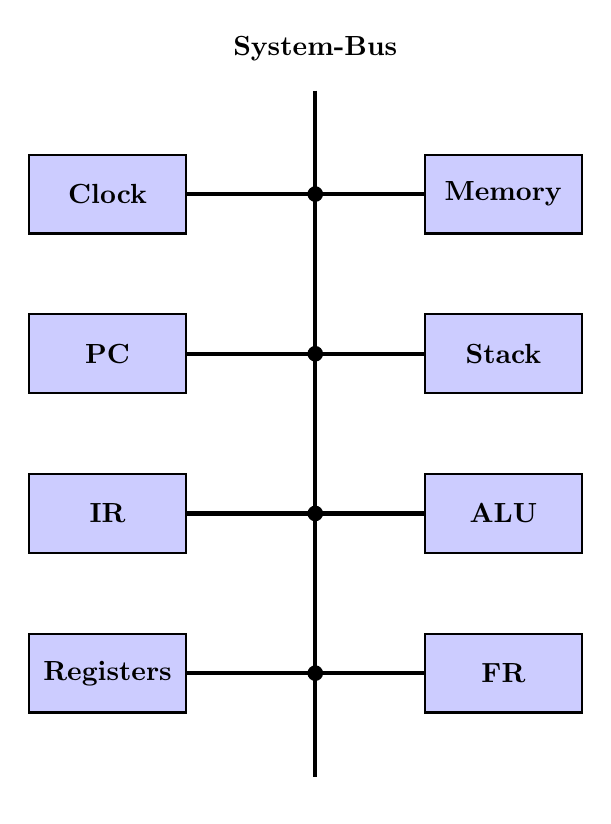
\begin{tikzpicture}
		[comp/.style = {thick, draw, rectangle, fill=blue!20!white, minimum width=2cm, minimum height=1cm},
		 int/.style = {fill=black, circle, inner sep=2pt}]
		\node[comp] (clock) {\textbf{Clock}};
		\node[comp, below=of clock] (pc) {\textbf{PC}};
		\node[comp, below=of pc] (ir) {\textbf{IR}};
		\node[comp, below=of ir] (reg) {\textbf{Registers}};
		\node[comp, right=3cm of clock] (mem) {\textbf{Memory}};
		\node[comp, below=of mem] (stack) {\textbf{Stack}};
		\node[comp, below=of stack] (alu) {\textbf{ALU}};
		\node[comp, below=of alu] (freg) {\textbf{FR}};
		\node[above right=0.8cm and 1.5cm of clock, label={\textbf{System-Bus}}] (busstart) {};
		\node[below right=0.8cm and 1.5cm of reg] (busend) {};

		\draw[ultra thick] (busstart) -- (busend);
		\draw[ultra thick] (clock) -- (busstart |- clock) node[int] {} -- (mem);
		\draw[ultra thick] (pc) -- (busstart |- pc) node[int] {} -- (stack);
		\draw[ultra thick] (ir) -- (busstart |- ir) node[int] {} -- (alu);
		\draw[ultra thick] (reg) -- (busstart |- reg) node[int] {} -- (freg);
	\end{tikzpicture}
	\caption{System architecture}
\end{figure}


\subsection*{Instruction Set}
\subsubsection*{General Overview}
The instruction set consists of 32 different instructions. The first 5 bit of the operation code are interpreted as the instruction. The instructions that have to implemented are the following:
\begin{table}[H]
	\centering
	\begin{longtable}{p{0.2\textwidth}p{0.02\textwidth}p{0.1\textwidth}p{0.68\textwidth}}
	\textbf{Data transfer}&\rownumber & LDW & Load a value of a memory address into a register\\
	&\rownumber & LDB & Load the LSB of a memory address into a register\\
	&\rownumber & MOVE & Move a value from one register to the next\\
	&\rownumber & STRW & Store the value of a register in a memory adress\\
	&\rownumber & STRB & Store the LSB of a register value in a memory address\\
	\end{longtable}
	\begin{longtable}{p{0.2\textwidth}p{0.02\textwidth}p{0.1\textwidth}p{0.68\textwidth}}
	\textbf{Stack}&\rownumber & PUSH & Push register value onto the stack\\
	&\rownumber & POP & Pop value from the stack\
	\end{longtable}
	\begin{longtable}{p{0.2\textwidth}p{0.02\textwidth}p{0.1\textwidth}p{0.68\textwidth}}
	\textbf{ALU}&\rownumber & ADD & Add the values of two registers\\
	&\rownumber & SUB & Subtract the values of two registers\\
	&\rownumber & AND & Bitwise AND of the values of two registers\\
	&\rownumber & OR & Bitwise OR of the values of two registers\\
	&\rownumber & NOT & Bitwise inversion of the value in one register\\
	&\rownumber & LSHIFT & Shift the value in one register to the left by a variable amount\\
	&\rownumber & RSHIFT & Shift the value in one register to the right by a variable amount\\
	&\rownumber & SIXT & Sign extension of the LSB\\
	\end{longtable}
\end{table}\noindent
The free adresses may be used for instructions that extend the functionality. For
example, instructions that take immediate values. The operation codes have the following
general layout:\par

\subsubsection*{Instruction Set Architecture}
\renewcommand{\arraystretch}{1.2}
\begin{center}
    \begin{longtable}{m{0.45\textwidth}m{0.12\textwidth}m{0.38\textwidth}}
        \textbf{Operation Code} & \textbf{Mnemonic} & \textbf{Description}\\
        \hlineB{2.2}
        \boxchar{0100 0001 0mmm 1nnn} & LDW       & Load the word that is stored at the
                                                    address held by the register
                                                    \texttt{Rmmm} into the register
                                                    \texttt{Rnnn}.\\
                                                    \hline
        \boxchar{0100 1001 0mmm 1nnn} & LDB       & Load the least significant byte of
                                                    the word at the address held by the
                                                    register \texttt{Rmmm} into the
                                                    register \texttt{Rnnn}.\\
                                                    \hline
        \boxchar{0101 0nnn bbbb bbbb} & MOVE      & Move the value
                                                    \texttt{bbbb'bbbb} into the register
                                                    \texttt{Rnnn}.\\
                                                    \hline
        \boxchar{0110 0001 0mmm 1nnn} & STRW      & Store the value of the register
                                                    \texttt{Rmmm} at the address held by
                                                    the register \texttt{Rnnn}.\\
                                                    \hline
        \boxchar{0110 1001 0mmm 1nnn} & STRB      & Store the least significant byte of
                                                    the value in register
                                                    \texttt{Rmmm} at the address held by
                                                    the register \texttt{Rnnn}.\\
                                                    \hline
        \boxchar{0000 00ps xxxx xxxx} & PUSH      & Push the declared registers \texttt{x}, the stack pointer \texttt{s} or the program counter \texttt{p} on the stack\\
        \hline
        \boxchar{0000 10ps xxxx xxxx} & POP       & Pop values from the stack in the declared registers \texttt{x}, the stack pointer \texttt{s} or the program counter \texttt{p}.\\
        \hline
        \boxchar{1000 001m mmnn nddd} & ADD       & Add the values of the registers
                                                    \texttt{Rmmm} and \texttt{Rnnn} and
                                                    store the result in the register
                                                    \texttt{Rddd}.\\
                                                    \hline
        \boxchar{1000 101m mmnn nddd} & SUB       & Subtract the value in the register
                                                    \texttt{Rnnn} from the value in
                                                    the register \texttt{Rmmm} and store
                                                    the result in the register
                                                    \texttt{Rddd}.\\
                                                    \hline
        \boxchar{1001 001m mmnn nddd} & AND       & Calculate a bitwise AND of the values in
                                                    the registers \texttt{Rmmm}
                                                    and \texttt{Rnnn}. Store the result
                                                    in the register \texttt{Rddd}.\\
                                                    \hline
        \boxchar{1001 101m mmnn nddd} & OR        & Calculate a bitwise OR of the values
                                                    in the registers \texttt{Rmmm} and
                                                    \texttt{Rnnn}. Store the result in
                                                    the register \texttt{Rddd}.\\
                                                    \hline
        \boxchar{1010 0001 0mmm 1ddd} & NOT       & Bitwise inversion of the value in
                                                    the register \texttt{Rmmm}. Store
                                                    the result in the register
                                                    \texttt{Rddd}.\\
                                                    \hline
        \boxchar{1010 1001 0mmm bbbb} & LSHIFT    & Shift the value in the register
                                                    \texttt{Rmmm} by \texttt{bbbb} to
                                                    the left.\\
                                                    \hline
        \boxchar{1011 0001 0mmm bbbb} & RSHIFT    & Shift the value in the register
                                                    \texttt{Rmmm} by \texttt{bbbb} to
                                                    the right.\\
                                                    \hline
        \boxchar{1011 1000 0000 1nnn} & SIXT      & Signextend the least significant
                                                    byte of the value that is stored
                                                    in the register \texttt{Rnnn}.\\
                                                    \hline
    \end{longtable}
\end{center}
\subsection*{ALU}
The ALU consists of the following components:
\begin{itemize}
    \item carry lookahead adder (CLAA)
    \item barrel shifter
    \item wallace tree multiplier
    \item logic unit
    \item flag register
\end{itemize}

\begin{tikzpicture}[]
    \node[lu] (lu) {};
    \node[claa, xshift=4cm] (claa) {};
    \node[wtmul, xshift=8cm] (claa) {};
\end{tikzpicture}

\end{document}
